\chapter{Design and Implementation of Slope}
\label{chap:design}


We present and discuss in depth the design and implementation of Slope, a migration framework which
satisfies the requirements and conditions discussed in \autoref{chap:migratableapps}.

\section{Design elements}
\label{sec:deselem}
Slope has to provide features such as transferring objects without serialization
and deserialization that are unusual in more generic systems.
Memory management is key to deliver these capabilities. Specifically, we must
carefully consider the problems of local memory layout, internal program memory
allocators, distributed memory management, and memory ownership tracking.

\subsection{Local memory layout}
\label{sec:localmem}
To eliminate the serialization and deserialization steps, we use a specific
memory layout to store migratable objects.
Similar to RAMP \cite{memon2018ramp}, each program instance reserves a
specific contiguous part of its virtual memory address space. The size of this
segment must be at least equal to the \emph{sum} of maximum physical memory that the
application plans to devote to migratable objects, which can be
as high as the total amount of physical memory in the cluster.
The starting address of this memory range is the same address on all machines.
This reservation is done at program initialization time
(i.e. before \texttt{main()}).

We will refer to this section of the virtual
address space as migratable memory or Slope memory. Note that mappings for
these pages are not yet generated and therefore the size of the Slope memory
region can be much larger than the amount of physical memory on a machine.

To synchronize accesses to memory during the migration process, we need a way
to control accesses to the pages in Slope memory. We therefore choose to manage
Slope memory by 4KB page granularity as this is the smallest unit of control
for setting memory page protection mappings. We also support other page sizes
if supported by the MMU and the OS (e.g., 2MB huge pages on x86/Linux).

\begin{figure}[t]
\centering
\ensurepdffromsvg{local-memory-management-phys-log.drawio}
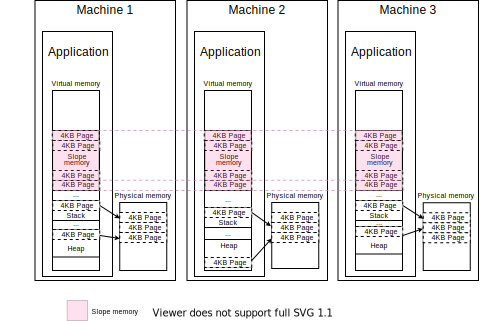
\includegraphics[width=1\textwidth]{local-memory-management-phys-log.drawio}
\caption{
    Placement of Slope memory on each node upon initialization.
}
\label{fig:localmemorymanagementphyslog}
\end{figure}

\autoref{fig:localmemorymanagementphyslog} shows how the local memory layouts
of the machines compare with each other. Notice how Slope memory is at the
same location in the virtual address space of the program on each node.
It also has the same size and page boundaries on all machines. Also note how
the 4KB pages from that region are not mapped to any physical memory pages
yet.

The placement of Slope memory in the application virtual address space is
central to the migration process. An object which only references addresses
within the Slope memory on one machine, can be moved to a different machine
and put on the same virtual address, page by page, along with the addresses
that it references and the object would continue to ``work'' in its new
residence. This in essence describes a migration operation and is how we will
eliminate the need to serialize and deserialize these objects.

Migrating objects to the same virtual addresses on different machines,
however, requires multiple conditions to be in place, and multiple
housekeeping tasks to be taken care of. For example the object must not have
any references to resources falling outside of the migratable memory. These
could be objects in non-migratable memory, or file descriptors, which refer
to resources beyond the scope of the application. Memory allocation
and deallocation must also be handled to prevent objects from overwriting each
others' pages during a migration.

Starting from the local memory layout, all of the design elements and
sub-systems in Slope are directed towards providing a migration API with the
requirements discussed in the previous chapter, while enabling us to deal with
the above
issues.


\subsubsection{Fundamental requirement of fixed addresses}
\label{sec:fixedfundamental}
\begin{figure}[tp]
\begin{lstlisting}
template<typename T> class ptr_hash;
template<typename T> class ptr_hash<T*> {
  using Type = T*;
 public:
  size_t operator()(const Type& ptr) const {
    return reinterpret_cast<std::uintptr_t>(ptr);
  }
};
int main() {
  std::unordered_map<int*, int, ptr_hash<int*>> the_map;
  std::vector<int> the_map(0);
  // Uncommenting will result in passing the assert
  // the_vector.reserve(2);
  the_vector.push_back(1);
  the_map[&the_vector[0]] = 1;
  the_vector.push_back(2);
  assert(*(the_map.begin()->first) == the_map.begin()->second); // fails
}
\end{lstlisting}
\caption{
    Referencing an object (int) through its virtual address
}
\label{fig:localmemorymanagementfundamental}
\end{figure}




Placing Slope memory on the same virtual address in all machines is,
unfortunately, a fundamental requirement. \autoref{fig:localmemorymanagementfundamental}
shows an example of why this is the case.

Lines $1-8$ show the creation of a hash
    function for pointers which simply uses their value, which is a virtual
    memory address. The vector needs to move the contents of its underlying
    array to a bigger array before inserting the second element at line $16$.

    At this point, from the viewpoint of
    \texttt{the\_map}, \texttt{the\_vector} has ``moved'', effectively shifting its start
    address to a new virtual address, but \texttt{the\_map} has no way of figuring out
    the new address and no way of translating its address dependencies.
    This means the address of the first element of \texttt{the\_vector} will
    change after executing line $16$, causing the assert in line $17$ to
    fail.

Uncommented, line $13$ would have ensured that the vector has
    allocated an underlying array that is big enough to hold 2 integers without
    the need to allocate a bigger array after the second \texttt{push\_back} in
    line $16$.






\begin{figure}[tp]
\begin{lstlisting}
int main() {
  std::unordered_map<int, int> the_map;
  std::vector<int> the_vector(0);
  the_vector.push_back(1);
  the_map[0] = 1;
  the_vector.push_back(2); // results in the_vector[0] being moved
  assert(the_vector[the_map.begin()->first] == the_map.begin()->second);
  // succeeds
}
\end{lstlisting}
\caption{
    Referencing an object (int) through its index
}
\label{fig:refbyindex}
\end{figure}


In contrast, had we stored indices instead of addresses in \texttt{the\_map},
allowing them to be translated to addresses internally, we could have prevented
the problem. \autoref{fig:refbyindex} demonstrates this approach. In this example,
the second call to \texttt{push\_back()} at line $6$ changes \texttt{\&the\_vector[0]},
however this will not pose a problem since no object depends on this address
value apart from \texttt{the\_vector}.

The implication is that as long as the
application has any means of referencing the underlying virtual address of any
of its resources, its correct execution may depend on that address
staying the same at every point during the execution of the program. Therefore
migrating an object without serialization and deserialization to another
machine (process)
requires byte by byte replication of its memory to the exact same virtual
addresses in the other machine (process) in the general case.

\subsection{Distributed memory management}
\label{sec:globalmem}
To simplify the discussion, from this point on we will assume that all of the
machines in the cluster have equal amounts of physical memory and that we want
to allow Slope to be able to use as much as all of the physical memory on each
machine.

Slope memory will therefore be of size $n \times m$ where $n$ is the number
of machines and $m$ is the physical memory available to each machine. We assign
the ownership of the first $m$ bytes of memory to the first machine, the
second $m$ bytes to the second machine and so on, such that the $i$th machine
owns the $i$th $\frac{1}{n}$ of Slope memory.

We can simplify the distributed allocation of memory if we only allow the
machines to allocate memory from the section that they own, however this may
result in memory address load imbalance. For example if one machine keeps
allocating objects and then quickly migrates them to the other machines, the
$\frac{1}{n}$ of the Slope memory belonging to this machine will soon run out,
and the machine will not be able to create any more migratable objects
even though the global Slope memory and the node's local physical memory are
far from full.

This requires us to devise a distributed memory management scheme which allows
us to use possibly all of the available Slope memory regardless of which
machine we are allocating the memory from, while avoiding clashes
between the allocated addresses across the cluster.


\begin{figure}[t]
\centering
\ensurepdffromsvg{leaserange.drawio}
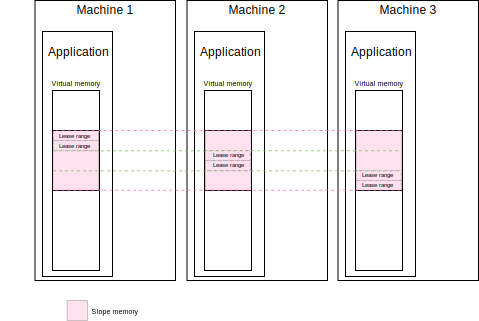
\includegraphics[width=1\textwidth]{leaserange.drawio}
\caption{
    Cluster memory layout and lease ranges
}
\label{fig:leaserange}
\end{figure}


We divide the Slope memory into sections that we call lease ranges. Each lease
range must be fully contained in one machine's $\frac{1}{n}$ of memory.
Lease ranges are the units of distributed ownership of Slope memory.
\autoref{fig:leaserange} shows placement of lease ranges
in Slope memory.


At any point, each lease range is owned by at most
one machine. Initially, none of the leases are held by any of the machines.
For the duration of the program, each machine is responsible for
the leases that initially fall in its $\frac{1}{n}$ of Slope memory.
That means the machine can hand out
the lease ownership to itself or other machines for any of the leases it is
responsible for.


Machines allocate virtual memory pages from the lease ranges they own. Initially
when
the machines do not own any leases to allocate from, or when the unallocated
memory in the
ranges that they already own does not suffice for their new allocations, they
need to ask for a new lease. To solve the memory imbalance problem, each node
will decide to direct its request for a new lease to the machine which
has the highest number of free leases based on its local information.
Each machine broadcasts information about their allocations, including
the number of free lease ranges to the cluster in preset intervals.

The length of the broadcast interval and the size of the lease ranges are two
parameters that we must choose based on the application. Shorter broadcast
intervals and smaller lease ranges will result in finer grain control over
how well we balance the memory allocations among the cluster machines.

In our experiments we set the lease sizes to 1GB and
make each machine broadcast its information every 1 second. In a 4 machine
setting and several memory allocation workloads, both values were small enough
to keep the maximum difference between the
allocated memory in any two machines to at most 2GB at all times.
Furthermore, varying the size from
500MBs to 5GBs and the interval from 0.5s to 5s did not yield any meaningful
difference in any of the observations.


The 1GB size allows for lease requests to be infrequent enough to amortize
seamlessly over the number of allocations, while keeping them small enough
to avoid sudden increases in the memory usage of any of the nodes. The 1
second interval keeps the lease ownership counts up to date across the cluster,
while causing little overhead to the application. However because of stale
information during the intervals, the nodes will not always
correctly choose the machine with the highest available lease count to allocate
from, but the 1GB size of the ranges which is relatively small compared to the
physical memory available to the machines will account for this inaccuracy.
This protocol
will keep the available number of leases in each machine roughly equal across
the cluster.

The above distributed memory allocation scheme not only eliminates the need for
a consensus box to track global memory allocations, but can also avoid
contention when multiple machines need to acquire new lease ranges with
little tweaks. For example each machine can randomly select to request the
lease from one of the top $k$ least occupied machines, instead of selecting
the least occupied machine, avoiding hotspots when multiple machines request
leases at the same time.

\subsection{Memory allocator}
\label{sec:platform}
We have chosen C++ as the platform to implement Slope, mainly because we need
to directly access process memory and manage the way it is allocated and used.
We implement \texttt{slope::memory::Allocator<T>} which is a memory allocator
conforming to the C++ allocator name requirement (e.g., providing
\texttt{allocate()} and \texttt{deallocate()}). It will internally satisfy the
local and global memory requirements of Slope following the protocols discussed
in \autoref{sec:localmem} and \autoref{sec:globalmem}.

\begin{figure}[t]
\begin{lstlisting}
template<typename T>
using MigratableUserDefinedType =
    UserDefinedType<T, slope::memory::Allocator<T>>;
\end{lstlisting}
\caption{
    Making predefined types migratable
}
\label{fig:migratableuserdefined}
\end{figure}

Any C++ type which accepts an allocator and uses it for all of its memory
allocations (i.e. \emph{AllocatorAwareContainer} \cite{cppnamedreqallocaware}
named requirement in the standard)
can be passed Slope's allocator. \autoref{fig:migratableuserdefined}
demonstrates how a preexisting well-written user-defined type can be
passed Slope's allocator without the need to change its internal implementation.

\begin{figure}[t]
\begin{lstlisting}
template<
    typename T,
    typename Allocator = std::allocator<T>
> class vector;
\end{lstlisting}
\caption{
    Declaration of \texttt{std::vector<T>}
}
\label{fig:stdvector}
\end{figure}


\begin{figure}[t]
\begin{lstlisting}
template<typename T>
using migratable_vector = std::vector<T, slope::memory::Allocator<T>>;

\end{lstlisting}
\caption{
    migratable \texttt{std::vector<T>}
}
\label{fig:migvector}
\end{figure}


With this design decision, STL containers (except \texttt{std::array} which
does not satisfy \texttt{AllocatorAwareContainer}) alongside many other preexisting
C++ structures can be easily made migratable.
For example \autoref{fig:stdvector} shows how the declaration of
\texttt{std::vector<T>}
allows the user to pass a custom allocator type. \autoref{fig:migvector} shows
how we can use the pattern in \autoref{fig:migratableuserdefined} to create
an alias for migratable vectors.



\begin{figure}[t]
\begin{lstlisting}
template<typename T, typename Allocator>
class UserDefinedType {
    static inline Allocator allocator;
    std::vector<T, Allocator> vector_;
    T *ptr_;
 public:
    template<typename... Args>
    UserDefinedType(Args&&... args):
      ptr_(new (allocator.allocate(1)) T(std::forward<Args>(args)...)) {}
    // ...
};
\end{lstlisting}
\caption{ Partial implementation of \texttt{UserDefinedType} which accepts an allocator}
\label{fig:userdefinedtype}
\end{figure}


A possible implementation for the \texttt{UserDefinedType} shown in
\autoref{fig:migratableuserdefined} might look like \autoref{fig:userdefinedtype}.
The class uses the allocator type passed to it to carry out any memory
allocations. Notice how the allocator can be conveniently passed down to the
class members (e.g., \texttt{std::vector<T, Allocator>}), showing the
composition-friendliness of using allocator classes that conform with C++ named
requirements.


\begin{figure}[tp]
\begin{lstlisting}
template <class T>
struct Allocator {
    // called after an object is received from a peer who migrated it
    // owner_addr: Address of the underlying T* object
    // memory_chunks: All segments of memory allocated under the
    //                object identified by owner_addr
    void adopt(owner_addr, memory_chunks) {
        for (chunk: memory_chunks) {
            add chunk to allocations of owner_addr
            set owner_addr as the owner of chunk
        }
    }

    // allocates memory of size n * sizeof(T) with the alginment of T
    T* allocate(std::size_t n) {
        current_object = top of contexts stack
        if (can fit the memory in one of the pages that the
                current_object already owns) {
            address = free memory from the page
        } else {
            while (owned lease ranges do not have enough space) {
                request new lease range
            }
            address = allocate memory pages from an owned lease range
        }
        Set the owner of address to be current object
        Add address to the ranges owned by the current object
        return address
    }
};
\end{lstlisting}
    \caption{ Outline of Slope memory allocator (Pseudo-code) }
\label{fig:allocimpl}
\end{figure}


\autoref{fig:allocimpl} shows an outline of the API and implementation of Slope's
memory allocator. The \texttt{adopt} function is called so that the memory
allocator can keep the information about a newly received object.
Should the object be migrated again, we need access to this information
to be able to perform the migration correctly. No memory is allocated during the call
to \texttt{adopt}.

On line 16 in the \texttt{allocate} function, the allocator infers
the owner of the memory that is being allocated to be the object whose
address is at the top of the context stack. This is how the allocator
associates virtual memory segments to the objects that own them. This is
discussed in detail in \autoref{sec:ownershiptracking}.



\subsection{Memory ownership tracking}
\label{sec:ownershiptracking}

\begin{figure}[tp]
\begin{lstlisting}
template <class T>
class mig_ptr {
 public:
    template<typename ...Args>
    mig_ptr(Args&& ...args);

    T *get();

    Context create_context();
};
\end{lstlisting}
    \caption{ Outline of \texttt{mig\_ptr}'s API }
\label{fig:migptrimpl}
\end{figure}


Passing Slope's memory allocator to types is not enough.
When an object is migrated to a different machine, we need to move all of the
memory that it references to the destination machine and put them at their
corresponding virtual memory addresses. This means
that we need a mechanism to keep track of the memory that an object owns.


We manage migratable objects through migratable pointers. The template\\
\texttt{slope::memory::mig\_ptr<T>} represents these types. A migratable
pointer works very similarly to a \texttt{std::unique\_ptr<T>}, with the
main distinction that it provides methods through which we can keep track
of the memory allocated by the underlying object.


\autoref{fig:migptrimpl} summarizes \texttt{mig\_ptr}'s API. Its
constructor forwards the arguments to
T's constructor(s), \texttt{get} retrieves the underlying object of
type \texttt{T*}, and most importantly \texttt{create\_context}
pushes the address of the underlying object to a thread local context stack.
The \texttt{allocate} function of the Slope allocator (\autoref{fig:allocimpl})
checks the top element of the context stack every time it is called to find out
which object we are allocating memory for. When the context object that
\texttt{create\_context} returns is destroyed (i.e. we go out of scope), the
context stack is also popped.


\begin{figure}[tp]
\begin{lstlisting}
using HashTablePartition = DistributedPartition<
    int, // key type
    int, // value type
    slope::memory::Allocator<int>
    >;
int main() {
    // underlying type uses slope::memory::Allocator
    // default constructor of HashTablePartition is used
    mig_ptr<HashTablePartition> partition;
    {
        // method called on mig_ptr
        auto context = partition.create_context();
        // get() gets the underlying pointer, put() inserts the value
        partition.get()->put("id", get_current_machine_id());
    } // context is invalidated as it goes out of scope
      // and destructor is called

    HashTableControlPlane<HashTablePartition> control_plane(
        [](mig_ptr<HashTablePartition> partition) {
            // No memory allocation possible in get; no context required
            // First get() gets the underlying pointer
            // Second get() queries the value in the partition
            std::cout << partition.get()->get("id") << std::endl;
        }
    );
    HashTableControlPlane.accept(partition);
    auto peer_id = get_current_machine_id() == "1" ? "0" : "1";
    auto mig_op = HashTableControlPlane.migrate(partition, peer_id);
    // carry out the migration using mig_op ...
    while (true) { /* wait */ }
}
\end{lstlisting}
\caption{
    usage of \texttt{create\_context()} method
}
\label{fig:migptrusage}
\end{figure}

\autoref{fig:migptrusage} corrects our early sketch in \autoref{fig:sketchmain}
to show how
ownership tracking and allocation context management fit with the control plane
API. For any method call
on type \texttt{T} that underlies the \texttt{slope::memory::mig\_ptr<T>},
if it has a possibility of calling \texttt{allocate()} on Slope allocator, it
must be enclosed in a \texttt{create\_context} call and the destruction of the
returned context. We call this behavior ``allocating memory for
an object''.

We keep a stack of contexts as they are created and destroyed by the application.
At each call to \texttt{allocate()}, the \texttt{mig\_ptr} whose context is at
the top of the stack will be set as the owner of the allocated memory.

Another important purpose that the \texttt{mig\_ptr} class template serves is
constructing the object itself. In addition to the memory allocations done
\emph{by} the object (e.g., allocating the underlying array by \texttt{std::vector}),
the object memory itself (e.g., \texttt{std::vector} object) must be placed in
migratable memory. This is an important step since we are not necessarily able
to construct the object elsewhere and then manually move it into the migratable
memory.


\subsection{Ownership management summary}
We will go over an example scenario to show how different layers of memory
ownership work together. Take the code snippet from \autoref{fig:migptrusage}
and assume it is being run on machine 1, in a cluster consisting of 3 machines.
Here is a possible course of events that we may observe on this machine.

First, the migratable pointer is created in \emph{non}-Slope memory. The
migratable pointer is only responsible for holding onto the migratable object
and does not need to be migratable itself. It will in turn try to allocate
Slope memory equal to the size of a \texttt{HashTablePartition} and constructs the
hash table in that memory.

Before the call to \texttt{allocate()} it creates
a temporary initialization context which we will later point to the object
that is about to be created. This is required because there is a circular
dependency between allocating the memory on which we are constructing the
hash table and setting the owner of that memory to be the hash table itself.
The circular dependency arises because we are not aware of the address of the
hash table before we allocate its memory.

After creating the initialization context, we call into \texttt{allocate()}.
None of the machines yet hold any lease ranges, so they will try to ask for one.
After looking at the current number of available lease ranges at each node,
they will choose one of the nodes in the cluster at random since all of them
have an equal number of available lease ranges. After being given
the ownership of a lease range we continue in the \texttt{allocate()} function.

We then allocate a page from the newly owned lease range on both machines (assuming the size of
a \texttt{HashTablePartition} is much less than a single memory page), and assign the
page and the allocated memory inside the page to the object that is being
created by breaking the circular dependency which is described above.
We return from the \texttt{allocate()} function and the initialization context
will be removed from the context stack.

We return from the constructor of the \texttt{HashTablePartition} and then
the migratable pointer. The call to \texttt{create\_context()} on line 12
will place each
\texttt{partition}'s context at the top of the context stack. As a consequence, all of the
Slope memory allocations will be assigned to \texttt{partition} until further change
to the context stack. We call into the \texttt{put()} member function, which
results in a call to \texttt{allocate()}. More memory will be allocated from
the page that embodies the \texttt{HashTablePartition} object since that page
still contains some empty space, otherwise for a large memory request we would
have allocated one or more new pages to accommodate the request.

With its context present at the top of
the context stack,
\texttt{partition} will own the newly allocated memory. Afterwards the context will
go out of scope, resulting in \texttt{partition}'s context being removed from the
context stack, leaving it empty. After the migrations take place, the \texttt{get()}
functions of the two partitions will be called, but they do not require
being enclosed in contexts as they do not allocate any memory.

\subsection{Choice of platform}
Allowing the application's data structures 
to rely directly on virtual memory addresses raises issues 
that we discussed in \ref{sec:deselem}. Many
of these could have been prevented if we had used a programming language such
as Java, which takes away this direct access, making the objects relocatable.

Even though Java provides certain features for portability and compatibility,
for some applications the overhead of being run in a managed environment
(e.g., under a garbage collector) is intolerable. A typical family of these
applications is distributed transaction
processing engines which includes Silo \cite{tu2013silo}, DrTM \cite{drtm2017},
and FaRM \cite{Dragojevic2014FaRM}. These are implemented in C++ to
reach the maximum possible performance and usually depend on lower level
components such as concurrent b-trees (e.g., Masstree \cite{mao2020masstree}).

Our motivation in using C++ for the design of Slope stems from the difficulty
of scaling such applications beyond a single node or designing them for a
multi-node cluster in the first place, and keeping the cluster load balanced.
The lower level dependencies of
these applications that may be optimized for single-node environments also
make it non-trivial to cross the gap from a single node to multiple nodes.

We design Slope for use in high performance applications where it is not
desirable to sacrifice performance to achieve load balancing and flexibility
in design. This means Slope provides a lower level function compared to
automatic serializability of objects in Java.
We can in fact use Slope to implement
an automatic layer of serializability or a migration platform in a higher
level language like Java with the possible added performance cost of running on
top of JVM. On the other hand, such a system can provide an API that is simpler
to use for the programmers since many of the house keeping tasks (e.g.,
\texttt{create\_context()}) are already done or partially taken care of by the JVM.


\section{Architecture}
At a high level, Slope consists of a control plane, responsible for carrying out
different phases of the migration operation and providing the means for the
servers to send and receive metadata to each other, an RDMA data plane
which handles sending and receiving memory pages,
and a specialized distributed memory management scheme, discussed in 
\autoref{sec:globalmem}. Slope's migration protocol is built atop these sub-systems.

% We have implemented the control plane and the data plane using
% RDMA over Infiniband because of how well the benefits of RDMA networking
% fit our problem specifications, but they can be implemented using any transport.

\subsection{Control plane}
The control plane provides an abstraction over which application instances can
execute migration operations and other side-tasks such as exchanging internal
system metadata or distributed memory allocation. For each operation we create
a reliable connected queue pair between each pair of machines, and pre-post to
them as many receive requests as we need to support concurrently. In our
experiments we found posting one read request for every core in the peer machine
will always prevent the sender from blocking.

Each machine immediately reposts
the consumed read request after receiving a completion, which further ensures
the presence of read requests at every queue end. After that a request
flow starts during which the two machines will go back and forth using other
established queue pairs to carry out the operation.

% Although
% the control plane can be practically replaced by any rpc framework, we do not
% have much to gain from using systems such as Herd \cite{kalia2016designguidelines} or
% FaSSt \cite{kalia2016fasst}, as the performance metrics in Slope are dominated
% mostly
% by the performance of the data plane.



% When using connected queue pairs, meta-data
% from each queue has to exist on the device cache for any operations to be
% carried out through that queue pair. As the number of queue pairs on each node
% increases linearly with the number of nodes in the cluster when we connect the
% QPs in a full-mesh manner, the performance of the application will collapse
% after we pass a certain number of nodes in the cluster, which has
% incentivized designs of RPC systems that use datagram queue pairs such as
% \cite{kalia2019datacenter} and \cite{kalia2016fasst}, even though others such
% as \cite{novakovic2019storm} have proposed hybrid one sided and two sided
% schemes which scale well. We have not reached a point where we can directly
% benefit from these optimizations as we are mostly throughput (data plane)
% limited. Furthermore we use each queue pair repeatedly in short bursts after a
% migration operation is triggered which avoids invalidating the ``active'' QP
% meta-data from the cache during the migration. However the control plane
% can be replaced entirely with any other RPC mechanism that achieves better
% performance.

% For co-ordination between machines (e.g., rendezvous protocol and transition
% to ready to send state)
% an out of band communication mechanism has to be used. We use memcached where 
% every node registers its queue pair and memory region parameters and
% information and waits to receive the same information from its peers. This
% phase only runs early in the program and does not have an effect on the
% performance of the system after the initialization is finished, at which point
% we no longer need the memcached server.

\subsection{Data plane}
The data plane is used to transfer contents of pages of Slope
memory from one machine to the same virtual page addresses in another node.
The role of the data plane is discussed in detail in \autoref{sec:migrationprotocol}.
It is responsible for the \emph{prefill} operation, during which it will
transfer pages of memory, but also keep track of any changes made to them on
the source, and the \emph{transfer} operation, which corrects the discrepancies
resulting from writes to the source memory during the prefill phase by
retransferring the affected pages.

% relaxed consistency requirements. Transfer operation follows shortly, during
% which we ensure the contents of the above memory section in the source are
% replicated to the same virtual addresses on the remote node. Prefilling is done
% in 4KB page granularity, while transfer can be done in larger units, depending
% on the contiguity of the memory section that is being transferred.

\label{migration_protocol_start_label}
\section{Migration protocol}
\label{sec:migrationprotocol}

\autoref{fig:migrationprotocol} outlines the migration protocol and the role
of Slope at different stages during the migration timeline.

\begin{figure}[tp]
\centering

\ensurepdffromsvg{migration-protocol.drawio}
\includegraphics[width=1\textwidth]{migration-protocol.drawio}
\caption{
    Slope migration protocol starting from object creation. Time progresses
    downwards.
    The steps illustrated here are described on pages \pageref{migration_protocol_start_label} to \pageref{migration_protocol_end_label}.
}
\label{fig:migrationprotocol}
\end{figure}

We observe the lifetime of a migratable data structure from the point it is
created until after we finish migrating it to another node.
Throughout the migration
there are certain conditions that need to be satisfied by the application
for the migration operation to finish correctly. We discuss these conditions
in detail alongside the steps in the migration protocol.

\subsubsection{Object creation}
During this phase the source machine calls into the Slope library multiple
times, based on how many times memory allocation and deallocation is required.

\paragraph{Source}
creates a migratable object, which we will refer to as the \emph{target object}.
Up until the point that
the source initiates the migration, all of the memory allocations of the target object
must happen through
Slope's custom memory allocator through allocation contexts as discussed in
\autoref{sec:ownershiptracking}.
The application must enclose the memory allocations of the migratable objects
with the correct allocation contexts to make sure Slope correctly keeps track of the
memory that each object references.

After the object is created the program will introduce the object to the
control plane using the \texttt{accept()} method of the control plane.
This may result in further calls to the memory allocator as
the object might need to allocate memory to process its incoming
requests or carry out the calls to its member functions.
Like any other memory allocation done on behalf of the object, these must
also be enclosed in contexts. At any point in time we would know which
memory pages belong to the target object.

\subsubsection{Migration initiation}
The application logic decides that the target object must be migrated from the
source machine to the destination. This might happen because the source machine
is balancing out its load by offloading the object to the destination or because
this particular object will benefit from running on the destination machine
by being local to resources that are available there.

This is the first time that the destination
machine will need to know about the properties of the target object. Had the
source machine not initiated the migration, the destination machine would have
stayed unaware of the existence of this object, while still avoiding
clashes on the allocated addresses across the cluster through the
use of lease ranges, as discussed in \autoref{sec:globalmem}.

\paragraph{Source}
initiates the migration by calling into Slope using the \texttt{migrate} method of the control plane. From this point
on, the application instance on the source machine should neither
cause any memory to be allocated to the target object, nor should it deallocate any memory that
this object references. Each of these can result from calling member functions
of the target object which either deallocate Slope memory previously held by the
object, or create Slope memory allocation contexts from the object and
use them to allocate Slope memory for the object.

The application is responsible
to ensure that these conditions hold. Currently Slope throws an exception if such
behavior is observed and for example in the case of \texttt{deallocate()}, the
escape of the exception from the function results in undefined behavior.
\autoref{sec:optim} briefly discusses how we can improve on this by relaxing
these requirements.

The \texttt{migrate} method returns a \texttt{MigrationOperation} object to
the caller. The application must use this object to carry out the migration.
This object is a wrapper around a concurrent state machine through which the
application code and Slope will coordinate to allow the object to be used on
the source for as long as possible.


\begin{figure}[tp]
\begin{lstlisting}
class MigrationOperation {
 public:
    bool try_finish_write();
    bool try_finish_read();
    int get_state();
};
\end{lstlisting}
\caption{
    Non blocking methods in \texttt{MigrationOperation}'s API
}
\label{fig:migop}
\end{figure}

\autoref{fig:migop} shows a selection of the API of a migration operation
object. Blocking counterparts of these methods also exist. Typically after
receiving this object the source will repeatedly call \texttt{try\_finish\_write()}.
If the call returns false, the application will do some more work involving
writes or reads and try again. After a successful call to \texttt{try\_finish\_write()}
a similiar scenario repeats where the application keeps calling into
\texttt{try\_finish\_read()} until success, while doing some readonly work in between
failures. After \texttt{try\_finish\_read()} is called successfully, the source
effectively turns over the ownership of the object to the destination.

Slope also keeps a reference to the migration object. From the viewpoint of
Slope, the blocking API of the migration object is more
useful. Slope reaches certain points in the migration process where it needs to wait
for the application to give up its read or write access. At those points Slope
will block until the application approves Slope to proceed by first giving up
its write and read access in order.

Slope posts a send request to the QP that is shared
between the source and the destination, initiating the migration.
With this request, the source will include $p$ the total number of
memory pages that the target object references. Note that Slope requires the
memory pages owned by the target object to stay the same during the migration
process after a call which initiates the migration, which means $p$ will be
constant throughout the process.

\paragraph{Destination}
receives a migration request along with $p$, the number of memory pages that the
target object owns and therefore need to
be transferred. The destination then populates another QP shared with the source
with $p$ receive requests, each corresponding to one of the virtual memory pages
that underlie the target object. We switch to a different QP
to allow concurrent migrations to happen between pairs of nodes. The destination
then goes on to notify the source that it can receive the description of the $p$
pages. The destination needs to know the virtual page addresses
to first create mappings for them and then pin them in physical memory so that their
physical address will stay the same throughout the migration, while the network
device writes to the pages by their physical address over DMA.

\paragraph{Source} receives the clear to send from the destination and sends the starting address
of each of the $p$ pages to the destination. 

\paragraph{Destination} waits for $p$ page addresses, and for each one of them, pins the
corresponding page in physical memory, so that the addresses that underlie the
target object can be used in RDMA read and write verbs. Notice how
``pro-active'' strategies that do not require knowledge of the page addresses
will not work, as pinning the
whole Slope memory in the physical memory will in the worst case, exhaust the
available physical memory on some nodes, and in the best case, result in large
amounts of wasted physical memory space. When the $p$ pages are pinned
and are ready to be the target of the RDMA verbs, the destination responds back,
signaling that it has pinned all of the required pages.

\subsubsection{Prefill}
The goal of the prefill phase is to warm up the destination machine's memory to
minimize the window of time during which neither of the two participating machines
own the target object. No machine can read from or write to the object during
that time. Therefore a long window with no owner means a long throughput
and latency hiccup as the application does not make any progress.

During the prefill phase we copy the target object to the destination over RDMA.
What makes it different from simply transferring the contents of memory is that
during the prefill operation, the source is still allowed to write to or read from
any location in the target object memory,
despite not having permission to change the memory layout of the object
in any way by allocating or deallocating memory. We optimistically do the above
transfer knowing that some of the pages might need to be retransferred as they
are written to by the source machine after they are sent to the destination.
We will refer to these pages as dirty pages. We go through the prefill phase,
hoping that the application on the source machine will be able to partially
function during this phase, while dirtying a small percentage of the pages.

\paragraph{Source} will need to prefill the pages one by one. For each page
we first protect it from write accesses such that it can be read safely
by the network device. We then use RDMA WRITE to send them to the destination.

After writing a page to the destination, any writes to it on the source will
invalidate its value on the destination and the page becomes dirty. We detect
this by keeping these pages protected from write accesses even after we
send them to the destination. When (if) the first write to a page is captured
using the signal handler, we lift the write protection from the page, allowing
future writes to go through, but making note of the dirtied page, such that
we can retransfer it later. Detailed discussion of these steps follows:

\subparagraph{Preparation:} At this point in the process, the source still
has ownership over the target object memory. This means we need to coordinate
the access to the pages to prevent simultaneous reads and writes. To do this,
the source uses \texttt{mprotect} to block write accesses to the page that
is currently being processed.

\subparagraph{Send:} The page that is being processed is posted to a
data plane QP shared between the source and the sink, to be written to
its corresponding virtual address in destination over RDMA.
Notice that we do not put the \texttt{PROT\_WRITE} permission
of the current page back after the RDMA SEND finishes, as we need to
detect the future writes which might dirty the page.

We assign a page access status to each page and set it to ``not writable''. A
thread running the signal handler (trapped there because its write access had
been blocked) will wait for this flag to be set to ``writable''
at the end of the RDMA operation. At that point it will proceed with putting
back the \texttt{PROT\_WRITE} flag.
At any point in time the clean pages will have their access status flag unset,
which is how we distinguish between the dirty and clean pages.

\subparagraph{Dirty page detection:}
This will be done using memory mapping protections and manually
handling signals that
are raised as a consequence of invalid accesses to the protected memory pages.

Applications use overridden behaviors for handling the \texttt{SIGSEGV} signal
to prevent the program from terminating on invalid memory references.
The \texttt{SIGSEGV} handler is installed at program start.
It is important to keep in mind that
\texttt{SIGSEGV} is delivered
to the \emph{same} thread whose current instruction reads or writes memory
from a page that does not have the required permissions.

To synchronize the access to each page of the target object,
we set the protection flags of each page to \texttt{PROT\_READ} before sending
it over RDMA. This prevents any writes from happening while RDMA WRITE
is in progress. These writes will result in a \texttt{SIGSEGV} signal being
raised because of an invalid memory reference, and the thread will start
executing our custom \texttt{SIGSEGV} handler.

Inside the signal handler, we make note of the accessed address that
caused the signal to be raised. We mark the page containing the address as
dirty. In the simplest case, the RDMA WRITE corresponding to this page has
previously finished. We update the protection flags of this page back
to \texttt{PROT\_READ | PROT\_WRITE}
to allow further writes to the addresses in this page to succeed.

Otherwise the RDMA WRITE is still in progress in which case we need to wait for the
RDMA WRITE to finish before adding the \texttt{PROT\_WRITE} permission flag to
the page. In our
implementation we use a status flag and a condition variable for each page
to manage its write accesses inside the signal handler. The status flag
corresponding to a page shows whether or not the RDMA operation on that page
has finished, hence allowing us to write to it, and the condition variable
is used to wake up the threads waiting for the status flag to be set.

Each thread will will block inside the signal handler until
the RDMA operation is finished. They will be notified about this through the
condition variable. When the first thread from the ones waiting inside the
signal handler acquires the lock on the condition, it needs to write to a
page that is marked clean, and does not have the \texttt{PROT\_WRITE}
permission yet. Therefore this thread sets the correct flag and marks the page as
dirty.

From this point on, no other thread writing to this address enters the
handler and the threads that were already waiting for the lock inside the
handler do not need
to carry out any other steps regarding the status flag and the page permissions
after acquiring the lock and they will
return from the handler without further action, allowing their previously
faulting write to succeed.
\autoref{fig:dirtydetection} shows the execution flow of application threads
and how they cooperate in dirty page detection in the prefill phase.

\begin{figure}[tp]
\centering

\ensurepdffromsvg{dirty-detection.drawio}
\includegraphics[width=1\textwidth]{dirty-detection.drawio}
\caption{
    Execution flow of different application threads during the migration of
    the 4KB page at \texttt{0xc000} which at some point in time becomes dirtied.
    Time progresses downwards and the prefill has been started before all of
    the events in the figure. Notice how thread t2 writes to the page after the
    RDMA transfer completes and the page is already marked dirty and writable.
}
\label{fig:dirtydetection}
\end{figure}

\subsubsection{Transfer of ownership}
\label{sec:transowner}
After the prefill phase Slope will wait for the application to give up its write
access to the object
with a call to \texttt{try\_finish\_write()}. Once Slope has reached
this state, \texttt{try\_finish\_write()} will return \emph{true} to the application,
and the application must not subsequently write to the object.
This means the state of the dirty pages of the object is now final and
Slope can retransfer them to the destination. When the
application eventually turns over the read access too (by a successful call
to \texttt{try\_finish\_read()}), the ownership is passed
to the destination allowing it to write to or read from the object,
as well as allocating or deallocating memory on behalf of it.

\paragraph{Destination} receives the completions for the prefill RDMA WRITEs.
That is because those WRITEs are done with immediate values which results
in completion entries being created for them. After the destination
receives the completion of the
last SEND, it will send a request back to the source, asking the source to
finally give up the ownership of the object.

\paragraph{Source} will need to successfully call
\texttt{try\_finish\_write()} and \texttt{try\_finish\_read()} (or their
blocking counterparts) to allow Slope to proceed with the migration.

Until the call to \texttt{try\_finish\_write()} succeeds, which only happens
after Slope completes the prefill phase, the application is
semantically allowed to write to the object pages, but ideally it will
transition to a ``pre-transfer'' mode after the initial migration
initiation. In this phase the application should try to do mostly read-only
accesses to avoid dirtying too many pages as this will cause the migration
to be done less efficiently with more pages that need to be transferred twice.

A call to \texttt{try\_finish\_read()} may succeed anytime after a call to
\texttt{try\_finish\_write()} returns \emph{true}. Timing this call depends on the
application. The earlier the source finishes the reads, the faster the
ownership is be given to the destination, but the destination can access the
object only partially until the dirty pages are retransferred. By delaying the
call, the source can maintain read-only access to the object for a longer time
and the destination will have more time to retransfer the dirty pages, but
transferring the ownership (and therefore write access) to the destination
will be delayed.

After the application gives up its read and write access to the object,
Slope will use the dirty
page tracking data to identify the dirty pages and send their addresses
to the destination. This message will also hand over the ownership
of the target object to the destination.

\paragraph{Destination} is notified that it has been given the ownership of
the object and is clear to call the \texttt{run\_()} function of the object,
but also needs to re-pull the dirty pages whose addresses are attached to the
request since the contents of these pages on the destination machine are
outdated.

Slope starts the above two processes concurrently. The destination machine
first sets
\texttt{PROT\_READ | PROT\_WRITE} access for the clean pages and
\texttt{PROT\_NONE} for the dirty pages. We put the dirty page addresses into 
a priority queue and fetch them from the source machine in order, giving
precedence to the pages which result in a
\texttt{SIGSEGV} being raised at the destination from an access by the
application. This means that the page has \texttt{PROT\_NONE} permission set and
is immediately required by an application thread. When the page is pulled using
RDMA READ, the page mapping flags will be updated to include read and write
permissions and any thread waiting for those pages can proceed. This is done
similar to how we do the dirty page detection on the source machine which was
discussed earlier.

\subsubsection{Post-transfer}
After the transfer is done, the state of the application will be
indistinguishable from a situation where we allocated the target object on
the destination machine from the start, if we deal with one final housekeeping
task.

\paragraph{Destination} will notify the source that it has READ all of the
dirty pages and that it no longer needs the source to keep the
pre-transfer content of the object memory.

\paragraph{Source} will wait to receive the above message at which point it
safely \texttt{munmap}s the memory underlying the ``old'' target object. At
this point the state on the source looks as if the target object had never existed
there.

\label{migration_protocol_end_label}

\section{Optimizations and Corner cases}
\label{sec:optim}
Multiple optimizations opportunities and housekeeping tasks have been omitted
from the earlier parts of this chapter. In this section we attend to these
subtle but important pieces.

\paragraph{Relaxing no allocation/deallocation rules during prefill:}
From migration initiation until the end of the prefill phase, we are allowing
the application to use the target object in a limited way, namely without
allocating or deallocating memory on behalf of it. This requirement can be
relaxed to allow full access to the object before committing the
migration, by noting the new allocations/deallocations before committing the
migration and communicating that information to the destination at that time.

\paragraph{C++ programming style to account for the prefill phase:}
\label{sec:conform}
Writing programs that can both respect and leverage the prefill phases
described previously is important to keep code readable. The application
programmer can encode the
conditions and requirements of the migration phase using C++ language features.
For example to represent the object after giving up the write access, one can
cast the target object to make it constant, disallowing the user from calling
the object methods that are not const-qualified.

\paragraph{Allocation strategies:} There are multiple ways to improve the memory
allocation performance. Since we need to allocate memory to objects in page
granularity, it is important to reduce fragmentation and wasted space,
otherwise the two will quickly pile up to decrease usable memory and increase
communication overhead.

Applications may want to provide their custom allocators on top of the Slope
allocator which allocates big regions from the shared address space. Given that
reducing the number of pages underlying an object is desirable, using a general
allocator inside Slope would not necessarily be useful. A general allocator
will instead optimize for putting multiple objects together, regardless of which
object owns which parts of the memory.

\paragraph{Deallocation:} Reasoning about and implementing deallocation must
be done with care since we have a local and a distributed level of memory
allocation in the system and multiple problems must be dealt with.

We need to handle deallocations both locally and globally. More concretely, we
need to correctly make note of the deallocated memory of each object, and also
keep track of the usage of each range lease such that they can be handed back
to their owners when they are no longer required.

Deallocation does not require an active context. Notice that requiring
an active context during deallocation is out of the question, since
deallocation could be happening in an object's destructor. This does not pose
a problem since we can keep an inverse map from memory allocations to
migratable objects and update it at each call to \texttt{allocate()}. We can
then use the inverse map to correctly attribute each deallocation with its
respective object and update the pages that underlie the object if necessary.

When a machine deallocates memory referenced by a migratable object, this
information needs to be sent back to the lease holder of the memory range in
which the deallocated memory falls. We do this off the critical path, such that
each meachine accumulates deallocated memories and sends them in batches to
the machines to which they originally belonged ($i$th $\frac{1}{n}$ of the
shared address space originally belongs to the $i$th machine), since the machine
on which the
deallocation happens does not have any information about
the actual lease owner of the embodying memory range. The original owner
of the memory range is then responsible to relay this information to the current
lease holder. If the machine on which the deallocation happens is already the
lease holder, we can avoid the extra round trip to the original owner of the
address and back to the lease holder.

The timings of these requests do not pose a problem. That is
because while deallocations can happen globally, allocations from a memory range
happen only at the owner and the order in which we interleave the two types of
operations cannot result in double deallocation (since each object is owned by
exactly one machine) and double allocation (since all of the allocations happen
at the current node on unallocated memory). The lease holder can turn the lease
over to the original owner if it does not contain any allocated memory.

\paragraph{Optimizing communication over RDMA:} There is room to optimize
the RDMA communication further. In some steps during the migration, we
increase the smallest unit of communication from pages to continuous chunks
of memory, possibly spanning multiple pages. Similarly when calling for
READs/WRITEs on continuous chunks or pages, we chain together multiple
WR's and post them in a single request to decrease the number of times we
have to notify the network device using MMIO over the PCIe bus.

In the prefill phase, instead of sending the full list of dirty pages to the
destination so that it can prioritize which of them to READ first, we can
proactively choose one or a small number of the pages and WRITE them in
parallel to sending the dirty list to the destination to save half of an rtt
in latency and leverage the free bandwidth.
For example we can prevent one page fault on the destination
if the page in which the allocated object \emph{reference} lies is dirty and
the source WRITEs it proactively, since this page will generate the first
fault when an object is accessed.


\paragraph{Multi-threading support:} Using Slope in a multi-threaded
environment does not require much extra effort. We need to use multiple
allocation context stacks and maintain them per thread, while maintaining
allocation mapping and inverse mapping globally. We therefore need to
synchronize accesses from multiple threads to these resources at certain points
in the \texttt{allocate()} and \texttt{deallocate()} functions.

Carrying out the migration operation through the \texttt{MigrationOperation}
in a multi-threaded environment is the responsibility of the application. E.g.,
The application on the source machine has to ensure that it stops all of
its threads from writing to the object before giving up the write access.

This concludes the design of Slope and the migration protocol at its core.
Next, we will show how Slope performs as a migration platforms in applications
with different needs.
